\documentclass[twoside]{book}

% Packages required by doxygen
\usepackage{fixltx2e}
\usepackage{calc}
\usepackage{doxygen}
\usepackage[export]{adjustbox} % also loads graphicx
\usepackage{graphicx}
\usepackage[utf8]{inputenc}
\usepackage{makeidx}
\usepackage{multicol}
\usepackage{multirow}
\PassOptionsToPackage{warn}{textcomp}
\usepackage{textcomp}
\usepackage[nointegrals]{wasysym}
\usepackage[table]{xcolor}

% Font selection
\usepackage[T1]{fontenc}
\usepackage[scaled=.90]{helvet}
\usepackage{courier}
\usepackage{amssymb}
\usepackage{sectsty}
\renewcommand{\familydefault}{\sfdefault}
\allsectionsfont{%
  \fontseries{bc}\selectfont%
  \color{darkgray}%
}
\renewcommand{\DoxyLabelFont}{%
  \fontseries{bc}\selectfont%
  \color{darkgray}%
}
\newcommand{\+}{\discretionary{\mbox{\scriptsize$\hookleftarrow$}}{}{}}

% Page & text layout
\usepackage{geometry}
\geometry{%
  a4paper,%
  top=2.5cm,%
  bottom=2.5cm,%
  left=2.5cm,%
  right=2.5cm%
}
\tolerance=750
\hfuzz=15pt
\hbadness=750
\setlength{\emergencystretch}{15pt}
\setlength{\parindent}{0cm}
\setlength{\parskip}{3ex plus 2ex minus 2ex}
\makeatletter
\renewcommand{\paragraph}{%
  \@startsection{paragraph}{4}{0ex}{-1.0ex}{1.0ex}{%
    \normalfont\normalsize\bfseries\SS@parafont%
  }%
}
\renewcommand{\subparagraph}{%
  \@startsection{subparagraph}{5}{0ex}{-1.0ex}{1.0ex}{%
    \normalfont\normalsize\bfseries\SS@subparafont%
  }%
}
\makeatother

% Headers & footers
\usepackage{fancyhdr}
\pagestyle{fancyplain}
\fancyhead[LE]{\fancyplain{}{\bfseries\thepage}}
\fancyhead[CE]{\fancyplain{}{}}
\fancyhead[RE]{\fancyplain{}{\bfseries\leftmark}}
\fancyhead[LO]{\fancyplain{}{\bfseries\rightmark}}
\fancyhead[CO]{\fancyplain{}{}}
\fancyhead[RO]{\fancyplain{}{\bfseries\thepage}}
\fancyfoot[LE]{\fancyplain{}{}}
\fancyfoot[CE]{\fancyplain{}{}}
\fancyfoot[RE]{\fancyplain{}{\bfseries\scriptsize Generated by Doxygen }}
\fancyfoot[LO]{\fancyplain{}{\bfseries\scriptsize Generated by Doxygen }}
\fancyfoot[CO]{\fancyplain{}{}}
\fancyfoot[RO]{\fancyplain{}{}}
\renewcommand{\footrulewidth}{0.4pt}
\renewcommand{\chaptermark}[1]{%
  \markboth{#1}{}%
}
\renewcommand{\sectionmark}[1]{%
  \markright{\thesection\ #1}%
}

% Indices & bibliography
\usepackage{natbib}
\usepackage[titles]{tocloft}
\setcounter{tocdepth}{3}
\setcounter{secnumdepth}{5}
\makeindex

% Hyperlinks (required, but should be loaded last)
\usepackage{ifpdf}
\ifpdf
  \usepackage[pdftex,pagebackref=true]{hyperref}
\else
  \usepackage[ps2pdf,pagebackref=true]{hyperref}
\fi
\hypersetup{%
  colorlinks=true,%
  linkcolor=blue,%
  citecolor=blue,%
  unicode%
}

% Custom commands
\newcommand{\clearemptydoublepage}{%
  \newpage{\pagestyle{empty}\cleardoublepage}%
}

\usepackage{caption}
\captionsetup{labelsep=space,justification=centering,font={bf},singlelinecheck=off,skip=4pt,position=top}

%===== C O N T E N T S =====

\begin{document}

% Titlepage & ToC
\hypersetup{pageanchor=false,
             bookmarksnumbered=true,
             pdfencoding=unicode
            }
\pagenumbering{roman}
\begin{titlepage}
\vspace*{7cm}
\begin{center}%
{\Large My Project }\\
\vspace*{1cm}
{\large Generated by Doxygen 1.8.11}\\
\end{center}
\end{titlepage}
\clearemptydoublepage
\tableofcontents
\clearemptydoublepage
\pagenumbering{arabic}
\hypersetup{pageanchor=true}

%--- Begin generated contents ---
\chapter{Class Index}
\section{Class List}
Here are the classes, structs, unions and interfaces with brief descriptions\+:\begin{DoxyCompactList}
\item\contentsline{section}{\hyperlink{structnode}{node} }{\pageref{structnode}}{}
\item\contentsline{section}{\hyperlink{structnode1}{node1} }{\pageref{structnode1}}{}
\item\contentsline{section}{\hyperlink{structnode__info}{node\+\_\+info} }{\pageref{structnode__info}}{}
\end{DoxyCompactList}

\chapter{File Index}
\section{File List}
Here is a list of all files with brief descriptions\+:\begin{DoxyCompactList}
\item\contentsline{section}{\hyperlink{Lab1_8c}{Lab1.\+c} }{\pageref{Lab1_8c}}{}
\end{DoxyCompactList}

\chapter{Class Documentation}
\hypertarget{classCommand}{}\section{Command Class Reference}
\label{classCommand}\index{Command@{Command}}


Collaboration diagram for Command\+:
\nopagebreak
\begin{figure}[H]
\begin{center}
\leavevmode
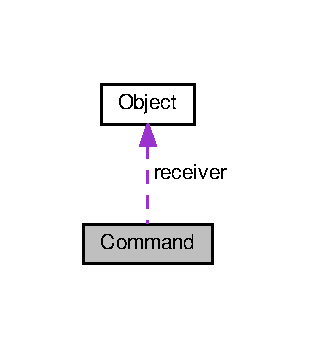
\includegraphics[width=149pt]{classCommand__coll__graph}
\end{center}
\end{figure}
\subsection*{Public Member Functions}
\begin{DoxyCompactItemize}
\item 
\hyperlink{classCommand_ab5004b23122fa06ca3613ee5d082ddc1}{Command} (\hyperlink{classObject}{Object} $\ast$new\+Receiver, \hyperlink{classCommand_a929c81cf8ef71dc52ef78156492f2a42}{Action} new\+Action)
\item 
virtual void \hyperlink{classCommand_a1f73a16e8706aec4c4db746f710b88d9}{execute} ()
\end{DoxyCompactItemize}
\subsection*{Static Public Member Functions}
\begin{DoxyCompactItemize}
\item 
static void \hyperlink{classCommand_a31a6d34a1d61f7cd994075a852714d3c}{undo} ()
\item 
static void \hyperlink{classCommand_ac807fae3326e22c02edc737708f9b288}{redo} ()
\end{DoxyCompactItemize}
\subsection*{Private Types}
\begin{DoxyCompactItemize}
\item 
typedef void(Object\+::$\ast$ \hyperlink{classCommand_a929c81cf8ef71dc52ef78156492f2a42}{Action}) ()
\end{DoxyCompactItemize}
\subsection*{Private Attributes}
\begin{DoxyCompactItemize}
\item 
\hyperlink{classObject}{Object} $\ast$ \hyperlink{classCommand_ac4a7e0c82bede3a8cd2f2b1478bd4763}{receiver}
\item 
\hyperlink{classCommand_a929c81cf8ef71dc52ef78156492f2a42}{Action} \hyperlink{classCommand_ac5473faf8b8b03ce83353838bc00c6dd}{action}
\end{DoxyCompactItemize}
\subsection*{Static Private Attributes}
\begin{DoxyCompactItemize}
\item 
static std\+::vector$<$ \hyperlink{classCommand}{Command} $\ast$ $>$ \hyperlink{classCommand_a3b694e6c1b5a3e62bdc0d7d1b3178eb1}{command\+List}
\item 
static std\+::vector$<$ \hyperlink{classMemento}{Memento} $\ast$ $>$ \hyperlink{classCommand_a03c855537275970db8e4b9c7ea64a9f9}{memento\+List}
\item 
static int \hyperlink{classCommand_a661b9cfc157529504ecf44528e4640b6}{num\+Commands} = 0
\item 
static int \hyperlink{classCommand_a06f1310ccbfdcfd18cfae03dcb428728}{max\+Commands} = 0
\end{DoxyCompactItemize}


\subsection{Member Typedef Documentation}
\index{Command@{Command}!Action@{Action}}
\index{Action@{Action}!Command@{Command}}
\subsubsection[{\texorpdfstring{Action}{Action}}]{\setlength{\rightskip}{0pt plus 5cm}typedef void(Object\+::$\ast$ Command\+::\+Action) ()\hspace{0.3cm}{\ttfamily [private]}}\hypertarget{classCommand_a929c81cf8ef71dc52ef78156492f2a42}{}\label{classCommand_a929c81cf8ef71dc52ef78156492f2a42}


\subsection{Constructor \& Destructor Documentation}
\index{Command@{Command}!Command@{Command}}
\index{Command@{Command}!Command@{Command}}
\subsubsection[{\texorpdfstring{Command(\+Object $\ast$new\+Receiver, Action new\+Action)}{Command(Object *newReceiver, Action newAction)}}]{\setlength{\rightskip}{0pt plus 5cm}Command\+::\+Command (
\begin{DoxyParamCaption}
\item[{{\bf Object} $\ast$}]{new\+Receiver, }
\item[{{\bf Action}}]{new\+Action}
\end{DoxyParamCaption}
)\hspace{0.3cm}{\ttfamily [inline]}}\hypertarget{classCommand_ab5004b23122fa06ca3613ee5d082ddc1}{}\label{classCommand_ab5004b23122fa06ca3613ee5d082ddc1}

\begin{DoxyCode}
59 : \hyperlink{classCommand_ac4a7e0c82bede3a8cd2f2b1478bd4763}{receiver} (newReceiver), \hyperlink{classCommand_ac5473faf8b8b03ce83353838bc00c6dd}{action} (newAction) \{\}
\end{DoxyCode}


\subsection{Member Function Documentation}
\index{Command@{Command}!execute@{execute}}
\index{execute@{execute}!Command@{Command}}
\subsubsection[{\texorpdfstring{execute()}{execute()}}]{\setlength{\rightskip}{0pt plus 5cm}virtual void Command\+::execute (
\begin{DoxyParamCaption}
{}
\end{DoxyParamCaption}
)\hspace{0.3cm}{\ttfamily [inline]}, {\ttfamily [virtual]}}\hypertarget{classCommand_a1f73a16e8706aec4c4db746f710b88d9}{}\label{classCommand_a1f73a16e8706aec4c4db746f710b88d9}

\begin{DoxyCode}
60                                \{
61             \textcolor{keywordflow}{if} (\hyperlink{classCommand_a03c855537275970db8e4b9c7ea64a9f9}{mementoList}.size() < \hyperlink{classCommand_a661b9cfc157529504ecf44528e4640b6}{numCommands} + 1)
62                 \hyperlink{classCommand_a03c855537275970db8e4b9c7ea64a9f9}{mementoList}.resize (\hyperlink{classCommand_a661b9cfc157529504ecf44528e4640b6}{numCommands} + 1);
63             \hyperlink{classCommand_a03c855537275970db8e4b9c7ea64a9f9}{mementoList}[\hyperlink{classCommand_a661b9cfc157529504ecf44528e4640b6}{numCommands}] = \hyperlink{classCommand_ac4a7e0c82bede3a8cd2f2b1478bd4763}{receiver}->
      \hyperlink{classObject_a169528dfd6ff33b21b038da8021cd748}{createMemento}();  \textcolor{comment}{// saves the last value}
64             \textcolor{keywordflow}{if} (\hyperlink{classCommand_a3b694e6c1b5a3e62bdc0d7d1b3178eb1}{commandList}.size() < \hyperlink{classCommand_a661b9cfc157529504ecf44528e4640b6}{numCommands} + 1)
65                 \hyperlink{classCommand_a3b694e6c1b5a3e62bdc0d7d1b3178eb1}{commandList}.resize (\hyperlink{classCommand_a661b9cfc157529504ecf44528e4640b6}{numCommands} + 1);
66             \hyperlink{classCommand_a3b694e6c1b5a3e62bdc0d7d1b3178eb1}{commandList}[\hyperlink{classCommand_a661b9cfc157529504ecf44528e4640b6}{numCommands}] = \textcolor{keyword}{this};  \textcolor{comment}{// saves the last command}
67             \textcolor{keywordflow}{if} (\hyperlink{classCommand_a661b9cfc157529504ecf44528e4640b6}{numCommands} > \hyperlink{classCommand_a06f1310ccbfdcfd18cfae03dcb428728}{maxCommands})
68                 \hyperlink{classCommand_a06f1310ccbfdcfd18cfae03dcb428728}{maxCommands} = \hyperlink{classCommand_a661b9cfc157529504ecf44528e4640b6}{numCommands};
69             \hyperlink{classCommand_a661b9cfc157529504ecf44528e4640b6}{numCommands}++;
70             (\hyperlink{classCommand_ac4a7e0c82bede3a8cd2f2b1478bd4763}{receiver}->*\hyperlink{classCommand_ac5473faf8b8b03ce83353838bc00c6dd}{action})();
71         \}
\end{DoxyCode}


Here is the call graph for this function\+:
\nopagebreak
\begin{figure}[H]
\begin{center}
\leavevmode
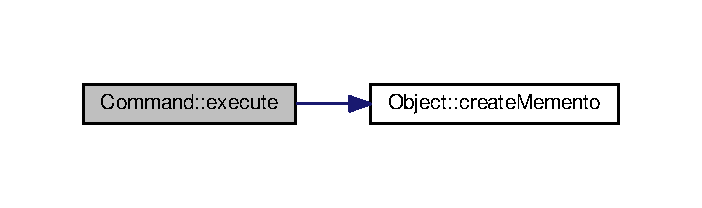
\includegraphics[width=337pt]{classCommand_a1f73a16e8706aec4c4db746f710b88d9_cgraph}
\end{center}
\end{figure}


\index{Command@{Command}!redo@{redo}}
\index{redo@{redo}!Command@{Command}}
\subsubsection[{\texorpdfstring{redo()}{redo()}}]{\setlength{\rightskip}{0pt plus 5cm}static void Command\+::redo (
\begin{DoxyParamCaption}
{}
\end{DoxyParamCaption}
)\hspace{0.3cm}{\ttfamily [inline]}, {\ttfamily [static]}}\hypertarget{classCommand_ac807fae3326e22c02edc737708f9b288}{}\label{classCommand_ac807fae3326e22c02edc737708f9b288}

\begin{DoxyCode}
81                            \{
82             \textcolor{keywordflow}{if} (\hyperlink{classCommand_a661b9cfc157529504ecf44528e4640b6}{numCommands} > \hyperlink{classCommand_a06f1310ccbfdcfd18cfae03dcb428728}{maxCommands})
83             \{
84                 std::cout << \textcolor{stringliteral}{"There is nothing to redo at this point."} << std::endl;
85                 return ;
86             \}
87             \hyperlink{classCommand}{Command}* commandRedo = \hyperlink{classCommand_a3b694e6c1b5a3e62bdc0d7d1b3178eb1}{commandList}[\hyperlink{classCommand_a661b9cfc157529504ecf44528e4640b6}{numCommands}];
88             (commandRedo->\hyperlink{classCommand_ac4a7e0c82bede3a8cd2f2b1478bd4763}{receiver}->*(commandRedo->\hyperlink{classCommand_ac5473faf8b8b03ce83353838bc00c6dd}{action}))();
89             \hyperlink{classCommand_a661b9cfc157529504ecf44528e4640b6}{numCommands}++;
90         \}
\end{DoxyCode}
\index{Command@{Command}!undo@{undo}}
\index{undo@{undo}!Command@{Command}}
\subsubsection[{\texorpdfstring{undo()}{undo()}}]{\setlength{\rightskip}{0pt plus 5cm}static void Command\+::undo (
\begin{DoxyParamCaption}
{}
\end{DoxyParamCaption}
)\hspace{0.3cm}{\ttfamily [inline]}, {\ttfamily [static]}}\hypertarget{classCommand_a31a6d34a1d61f7cd994075a852714d3c}{}\label{classCommand_a31a6d34a1d61f7cd994075a852714d3c}

\begin{DoxyCode}
72                            \{
73             \textcolor{keywordflow}{if} (\hyperlink{classCommand_a661b9cfc157529504ecf44528e4640b6}{numCommands} == 0)
74             \{
75                 std::cout << \textcolor{stringliteral}{"There is nothing to undo at this point."} << std::endl;
76                 \textcolor{keywordflow}{return};
77             \}
78             \hyperlink{classCommand_a3b694e6c1b5a3e62bdc0d7d1b3178eb1}{commandList}[\hyperlink{classCommand_a661b9cfc157529504ecf44528e4640b6}{numCommands} - 1]->receiver->reinstateMemento (
      \hyperlink{classCommand_a03c855537275970db8e4b9c7ea64a9f9}{mementoList}[\hyperlink{classCommand_a661b9cfc157529504ecf44528e4640b6}{numCommands} - 1]);
79             \hyperlink{classCommand_a661b9cfc157529504ecf44528e4640b6}{numCommands}--;
80         \}
\end{DoxyCode}


\subsection{Member Data Documentation}
\index{Command@{Command}!action@{action}}
\index{action@{action}!Command@{Command}}
\subsubsection[{\texorpdfstring{action}{action}}]{\setlength{\rightskip}{0pt plus 5cm}{\bf Action} Command\+::action\hspace{0.3cm}{\ttfamily [private]}}\hypertarget{classCommand_ac5473faf8b8b03ce83353838bc00c6dd}{}\label{classCommand_ac5473faf8b8b03ce83353838bc00c6dd}
\index{Command@{Command}!command\+List@{command\+List}}
\index{command\+List@{command\+List}!Command@{Command}}
\subsubsection[{\texorpdfstring{command\+List}{commandList}}]{\setlength{\rightskip}{0pt plus 5cm}std\+::vector$<$ {\bf Command} $\ast$ $>$ Command\+::command\+List\hspace{0.3cm}{\ttfamily [static]}, {\ttfamily [private]}}\hypertarget{classCommand_a3b694e6c1b5a3e62bdc0d7d1b3178eb1}{}\label{classCommand_a3b694e6c1b5a3e62bdc0d7d1b3178eb1}
\index{Command@{Command}!max\+Commands@{max\+Commands}}
\index{max\+Commands@{max\+Commands}!Command@{Command}}
\subsubsection[{\texorpdfstring{max\+Commands}{maxCommands}}]{\setlength{\rightskip}{0pt plus 5cm}int Command\+::max\+Commands = 0\hspace{0.3cm}{\ttfamily [static]}, {\ttfamily [private]}}\hypertarget{classCommand_a06f1310ccbfdcfd18cfae03dcb428728}{}\label{classCommand_a06f1310ccbfdcfd18cfae03dcb428728}
\index{Command@{Command}!memento\+List@{memento\+List}}
\index{memento\+List@{memento\+List}!Command@{Command}}
\subsubsection[{\texorpdfstring{memento\+List}{mementoList}}]{\setlength{\rightskip}{0pt plus 5cm}std\+::vector$<$ {\bf Memento} $\ast$ $>$ Command\+::memento\+List\hspace{0.3cm}{\ttfamily [static]}, {\ttfamily [private]}}\hypertarget{classCommand_a03c855537275970db8e4b9c7ea64a9f9}{}\label{classCommand_a03c855537275970db8e4b9c7ea64a9f9}
\index{Command@{Command}!num\+Commands@{num\+Commands}}
\index{num\+Commands@{num\+Commands}!Command@{Command}}
\subsubsection[{\texorpdfstring{num\+Commands}{numCommands}}]{\setlength{\rightskip}{0pt plus 5cm}int Command\+::num\+Commands = 0\hspace{0.3cm}{\ttfamily [static]}, {\ttfamily [private]}}\hypertarget{classCommand_a661b9cfc157529504ecf44528e4640b6}{}\label{classCommand_a661b9cfc157529504ecf44528e4640b6}
\index{Command@{Command}!receiver@{receiver}}
\index{receiver@{receiver}!Command@{Command}}
\subsubsection[{\texorpdfstring{receiver}{receiver}}]{\setlength{\rightskip}{0pt plus 5cm}{\bf Object}$\ast$ Command\+::receiver\hspace{0.3cm}{\ttfamily [private]}}\hypertarget{classCommand_ac4a7e0c82bede3a8cd2f2b1478bd4763}{}\label{classCommand_ac4a7e0c82bede3a8cd2f2b1478bd4763}


The documentation for this class was generated from the following file\+:\begin{DoxyCompactItemize}
\item 
\hyperlink{Memento_8cpp}{Memento.\+cpp}\end{DoxyCompactItemize}

\hypertarget{classMemento}{}\section{Memento Class Reference}
\label{classMemento}\index{Memento@{Memento}}


Collaboration diagram for Memento\+:
\nopagebreak
\begin{figure}[H]
\begin{center}
\leavevmode
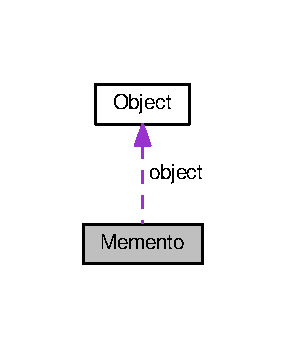
\includegraphics[width=139pt]{classMemento__coll__graph}
\end{center}
\end{figure}
\subsection*{Public Member Functions}
\begin{DoxyCompactItemize}
\item 
\hyperlink{classMemento_a7dc174ba544a54a0258aee0178f00619}{Memento} (const \hyperlink{classObject}{Object} \&obj)
\item 
\hyperlink{classObject}{Object} \hyperlink{classMemento_a13c0885085d6010835ebcfde5808f4af}{snapshot} () const 
\end{DoxyCompactItemize}
\subsection*{Private Attributes}
\begin{DoxyCompactItemize}
\item 
\hyperlink{classObject}{Object} \hyperlink{classMemento_ae264f38394a414c42f9e4315f2c25916}{object}
\end{DoxyCompactItemize}


\subsection{Constructor \& Destructor Documentation}
\index{Memento@{Memento}!Memento@{Memento}}
\index{Memento@{Memento}!Memento@{Memento}}
\subsubsection[{\texorpdfstring{Memento(const Object \&obj)}{Memento(const Object &obj)}}]{\setlength{\rightskip}{0pt plus 5cm}Memento\+::\+Memento (
\begin{DoxyParamCaption}
\item[{const {\bf Object} \&}]{obj}
\end{DoxyParamCaption}
)\hspace{0.3cm}{\ttfamily [inline]}}\hypertarget{classMemento_a7dc174ba544a54a0258aee0178f00619}{}\label{classMemento_a7dc174ba544a54a0258aee0178f00619}

\begin{DoxyCode}
37 :  \hyperlink{classMemento_ae264f38394a414c42f9e4315f2c25916}{object} (obj) \{\}
\end{DoxyCode}


\subsection{Member Function Documentation}
\index{Memento@{Memento}!snapshot@{snapshot}}
\index{snapshot@{snapshot}!Memento@{Memento}}
\subsubsection[{\texorpdfstring{snapshot() const }{snapshot() const }}]{\setlength{\rightskip}{0pt plus 5cm}{\bf Object} Memento\+::snapshot (
\begin{DoxyParamCaption}
{}
\end{DoxyParamCaption}
) const\hspace{0.3cm}{\ttfamily [inline]}}\hypertarget{classMemento_a13c0885085d6010835ebcfde5808f4af}{}\label{classMemento_a13c0885085d6010835ebcfde5808f4af}

\begin{DoxyCode}
38 \{\textcolor{keywordflow}{return} \hyperlink{classMemento_ae264f38394a414c42f9e4315f2c25916}{object};\}  \textcolor{comment}{// want a snapshot of Object itself because of its many data members}
\end{DoxyCode}


\subsection{Member Data Documentation}
\index{Memento@{Memento}!object@{object}}
\index{object@{object}!Memento@{Memento}}
\subsubsection[{\texorpdfstring{object}{object}}]{\setlength{\rightskip}{0pt plus 5cm}{\bf Object} Memento\+::object\hspace{0.3cm}{\ttfamily [private]}}\hypertarget{classMemento_ae264f38394a414c42f9e4315f2c25916}{}\label{classMemento_ae264f38394a414c42f9e4315f2c25916}


The documentation for this class was generated from the following file\+:\begin{DoxyCompactItemize}
\item 
\hyperlink{Memento_8cpp}{Memento.\+cpp}\end{DoxyCompactItemize}

\hypertarget{classObject}{}\section{Object Class Reference}
\label{classObject}\index{Object@{Object}}
\subsection*{Public Member Functions}
\begin{DoxyCompactItemize}
\item 
\hyperlink{classObject_ae6203b4273493f4aa9177445264d3272}{Object} (int new\+Value)
\item 
void \hyperlink{classObject_a7e43ddd2f4647f67ba9d6f18dd24bf77}{double\+Value} ()
\item 
void \hyperlink{classObject_a406add870a5642dc0d931aec975288f9}{increase\+By\+One} ()
\item 
int \hyperlink{classObject_afb7a055f066071c9abae831e9e9485e7}{get\+Value} () const 
\item 
std\+::string \hyperlink{classObject_a6390f4fca865dc59e3442e9f0fb6bd5e}{get\+Name} () const 
\item 
double \hyperlink{classObject_a20acb478a579d175f3e6ee6f4354577b}{get\+Decimal} () const 
\item 
\hyperlink{classMemento}{Memento} $\ast$ \hyperlink{classObject_a169528dfd6ff33b21b038da8021cd748}{create\+Memento} () const 
\item 
void \hyperlink{classObject_a19d41bf5b99d4a5880aaab5640d8787a}{reinstate\+Memento} (\hyperlink{classMemento}{Memento} $\ast$mem)
\end{DoxyCompactItemize}
\subsection*{Private Attributes}
\begin{DoxyCompactItemize}
\item 
int \hyperlink{classObject_aff40b305580fdacdf3e2c63dfc181152}{value}
\item 
std\+::string \hyperlink{classObject_a24457e0a387492c80594aec7681a2277}{name}
\item 
double \hyperlink{classObject_abee4fc3561439ea77b960f839f5c8616}{decimal}
\end{DoxyCompactItemize}


\subsection{Constructor \& Destructor Documentation}
\index{Object@{Object}!Object@{Object}}
\index{Object@{Object}!Object@{Object}}
\subsubsection[{\texorpdfstring{Object(int new\+Value)}{Object(int newValue)}}]{\setlength{\rightskip}{0pt plus 5cm}Object\+::\+Object (
\begin{DoxyParamCaption}
\item[{int}]{new\+Value}
\end{DoxyParamCaption}
)\hspace{0.3cm}{\ttfamily [inline]}}\hypertarget{classObject_ae6203b4273493f4aa9177445264d3272}{}\label{classObject_ae6203b4273493f4aa9177445264d3272}

\begin{DoxyCode}
23 : \hyperlink{classObject_aff40b305580fdacdf3e2c63dfc181152}{value} (newValue), \hyperlink{classObject_a24457e0a387492c80594aec7681a2277}{name} (\hyperlink{Memento_8cpp_a549853b5d8df8cf60e8d275a4df73b54}{NAME} + \hyperlink{Memento_8cpp_a90503872144928016292aaa273e07678}{toString} (\hyperlink{classObject_aff40b305580fdacdf3e2c63dfc181152}{value})), 
      \hyperlink{classObject_abee4fc3561439ea77b960f839f5c8616}{decimal} ((\textcolor{keywordtype}{float})\hyperlink{classObject_aff40b305580fdacdf3e2c63dfc181152}{value} / 100) \{\}
\end{DoxyCode}


\subsection{Member Function Documentation}
\index{Object@{Object}!create\+Memento@{create\+Memento}}
\index{create\+Memento@{create\+Memento}!Object@{Object}}
\subsubsection[{\texorpdfstring{create\+Memento() const }{createMemento() const }}]{\setlength{\rightskip}{0pt plus 5cm}{\bf Memento} $\ast$ Object\+::create\+Memento (
\begin{DoxyParamCaption}
{}
\end{DoxyParamCaption}
) const}\hypertarget{classObject_a169528dfd6ff33b21b038da8021cd748}{}\label{classObject_a169528dfd6ff33b21b038da8021cd748}

\begin{DoxyCode}
41                                      \{
42     \textcolor{keywordflow}{return} \textcolor{keyword}{new} \hyperlink{classMemento}{Memento} (*\textcolor{keyword}{this});
43 \}
\end{DoxyCode}
\index{Object@{Object}!double\+Value@{double\+Value}}
\index{double\+Value@{double\+Value}!Object@{Object}}
\subsubsection[{\texorpdfstring{double\+Value()}{doubleValue()}}]{\setlength{\rightskip}{0pt plus 5cm}void Object\+::double\+Value (
\begin{DoxyParamCaption}
{}
\end{DoxyParamCaption}
)\hspace{0.3cm}{\ttfamily [inline]}}\hypertarget{classObject_a7e43ddd2f4647f67ba9d6f18dd24bf77}{}\label{classObject_a7e43ddd2f4647f67ba9d6f18dd24bf77}

\begin{DoxyCode}
24 \{\hyperlink{classObject_aff40b305580fdacdf3e2c63dfc181152}{value} = 2 * \hyperlink{classObject_aff40b305580fdacdf3e2c63dfc181152}{value};  \hyperlink{classObject_a24457e0a387492c80594aec7681a2277}{name} = \hyperlink{Memento_8cpp_a549853b5d8df8cf60e8d275a4df73b54}{NAME} + \hyperlink{Memento_8cpp_a90503872144928016292aaa273e07678}{toString} (\hyperlink{classObject_aff40b305580fdacdf3e2c63dfc181152}{value});  
      \hyperlink{classObject_abee4fc3561439ea77b960f839f5c8616}{decimal} = (float)\hyperlink{classObject_aff40b305580fdacdf3e2c63dfc181152}{value} / 100;\}
\end{DoxyCode}


Here is the call graph for this function\+:
\nopagebreak
\begin{figure}[H]
\begin{center}
\leavevmode
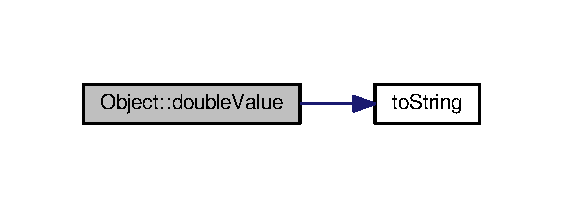
\includegraphics[width=270pt]{classObject_a7e43ddd2f4647f67ba9d6f18dd24bf77_cgraph}
\end{center}
\end{figure}


\index{Object@{Object}!get\+Decimal@{get\+Decimal}}
\index{get\+Decimal@{get\+Decimal}!Object@{Object}}
\subsubsection[{\texorpdfstring{get\+Decimal() const }{getDecimal() const }}]{\setlength{\rightskip}{0pt plus 5cm}double Object\+::get\+Decimal (
\begin{DoxyParamCaption}
{}
\end{DoxyParamCaption}
) const\hspace{0.3cm}{\ttfamily [inline]}}\hypertarget{classObject_a20acb478a579d175f3e6ee6f4354577b}{}\label{classObject_a20acb478a579d175f3e6ee6f4354577b}

\begin{DoxyCode}
28 \{\textcolor{keywordflow}{return} \hyperlink{classObject_abee4fc3561439ea77b960f839f5c8616}{decimal};\}
\end{DoxyCode}


Here is the call graph for this function\+:
\nopagebreak
\begin{figure}[H]
\begin{center}
\leavevmode
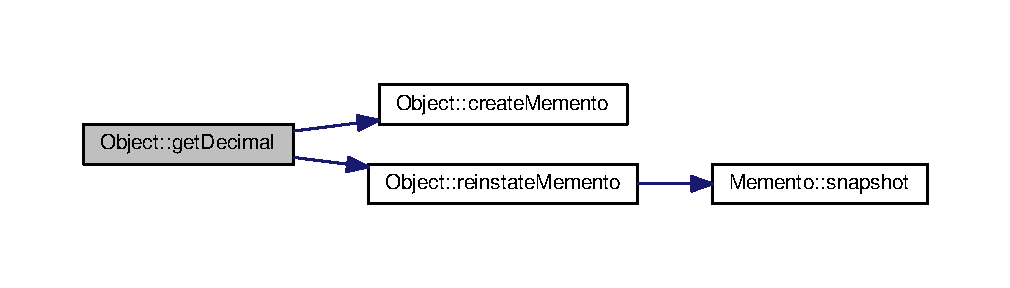
\includegraphics[width=350pt]{classObject_a20acb478a579d175f3e6ee6f4354577b_cgraph}
\end{center}
\end{figure}


\index{Object@{Object}!get\+Name@{get\+Name}}
\index{get\+Name@{get\+Name}!Object@{Object}}
\subsubsection[{\texorpdfstring{get\+Name() const }{getName() const }}]{\setlength{\rightskip}{0pt plus 5cm}std\+::string Object\+::get\+Name (
\begin{DoxyParamCaption}
{}
\end{DoxyParamCaption}
) const\hspace{0.3cm}{\ttfamily [inline]}}\hypertarget{classObject_a6390f4fca865dc59e3442e9f0fb6bd5e}{}\label{classObject_a6390f4fca865dc59e3442e9f0fb6bd5e}

\begin{DoxyCode}
27 \{\textcolor{keywordflow}{return} \hyperlink{classObject_a24457e0a387492c80594aec7681a2277}{name};\}
\end{DoxyCode}
\index{Object@{Object}!get\+Value@{get\+Value}}
\index{get\+Value@{get\+Value}!Object@{Object}}
\subsubsection[{\texorpdfstring{get\+Value() const }{getValue() const }}]{\setlength{\rightskip}{0pt plus 5cm}int Object\+::get\+Value (
\begin{DoxyParamCaption}
{}
\end{DoxyParamCaption}
) const\hspace{0.3cm}{\ttfamily [inline]}}\hypertarget{classObject_afb7a055f066071c9abae831e9e9485e7}{}\label{classObject_afb7a055f066071c9abae831e9e9485e7}

\begin{DoxyCode}
26 \{\textcolor{keywordflow}{return} \hyperlink{classObject_aff40b305580fdacdf3e2c63dfc181152}{value};\}
\end{DoxyCode}
\index{Object@{Object}!increase\+By\+One@{increase\+By\+One}}
\index{increase\+By\+One@{increase\+By\+One}!Object@{Object}}
\subsubsection[{\texorpdfstring{increase\+By\+One()}{increaseByOne()}}]{\setlength{\rightskip}{0pt plus 5cm}void Object\+::increase\+By\+One (
\begin{DoxyParamCaption}
{}
\end{DoxyParamCaption}
)\hspace{0.3cm}{\ttfamily [inline]}}\hypertarget{classObject_a406add870a5642dc0d931aec975288f9}{}\label{classObject_a406add870a5642dc0d931aec975288f9}

\begin{DoxyCode}
25 \{\hyperlink{classObject_aff40b305580fdacdf3e2c63dfc181152}{value}++;  \hyperlink{classObject_a24457e0a387492c80594aec7681a2277}{name} = \hyperlink{Memento_8cpp_a549853b5d8df8cf60e8d275a4df73b54}{NAME} + \hyperlink{Memento_8cpp_a90503872144928016292aaa273e07678}{toString} (\hyperlink{classObject_aff40b305580fdacdf3e2c63dfc181152}{value});  \hyperlink{classObject_abee4fc3561439ea77b960f839f5c8616}{decimal} = (float)
      \hyperlink{classObject_aff40b305580fdacdf3e2c63dfc181152}{value} / 100;\}
\end{DoxyCode}


Here is the call graph for this function\+:
\nopagebreak
\begin{figure}[H]
\begin{center}
\leavevmode
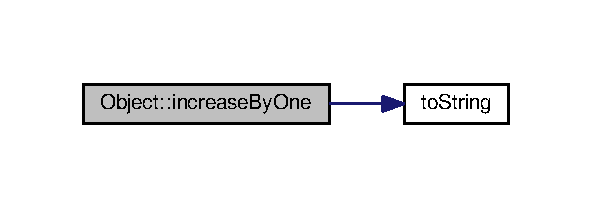
\includegraphics[width=284pt]{classObject_a406add870a5642dc0d931aec975288f9_cgraph}
\end{center}
\end{figure}


\index{Object@{Object}!reinstate\+Memento@{reinstate\+Memento}}
\index{reinstate\+Memento@{reinstate\+Memento}!Object@{Object}}
\subsubsection[{\texorpdfstring{reinstate\+Memento(\+Memento $\ast$mem)}{reinstateMemento(Memento *mem)}}]{\setlength{\rightskip}{0pt plus 5cm}void Object\+::reinstate\+Memento (
\begin{DoxyParamCaption}
\item[{{\bf Memento} $\ast$}]{mem}
\end{DoxyParamCaption}
)}\hypertarget{classObject_a19d41bf5b99d4a5880aaab5640d8787a}{}\label{classObject_a19d41bf5b99d4a5880aaab5640d8787a}

\begin{DoxyCode}
45                                            \{
46     *\textcolor{keyword}{this} = mem->\hyperlink{classMemento_a13c0885085d6010835ebcfde5808f4af}{snapshot}();
47 \}
\end{DoxyCode}


Here is the call graph for this function\+:
\nopagebreak
\begin{figure}[H]
\begin{center}
\leavevmode
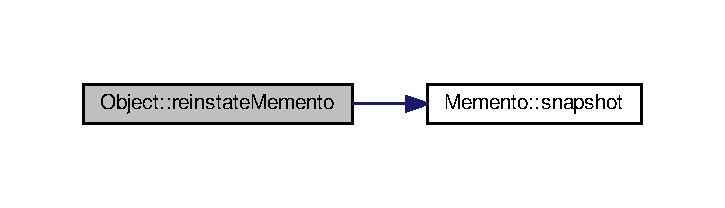
\includegraphics[width=348pt]{classObject_a19d41bf5b99d4a5880aaab5640d8787a_cgraph}
\end{center}
\end{figure}




\subsection{Member Data Documentation}
\index{Object@{Object}!decimal@{decimal}}
\index{decimal@{decimal}!Object@{Object}}
\subsubsection[{\texorpdfstring{decimal}{decimal}}]{\setlength{\rightskip}{0pt plus 5cm}double Object\+::decimal\hspace{0.3cm}{\ttfamily [private]}}\hypertarget{classObject_abee4fc3561439ea77b960f839f5c8616}{}\label{classObject_abee4fc3561439ea77b960f839f5c8616}
\index{Object@{Object}!name@{name}}
\index{name@{name}!Object@{Object}}
\subsubsection[{\texorpdfstring{name}{name}}]{\setlength{\rightskip}{0pt plus 5cm}std\+::string Object\+::name\hspace{0.3cm}{\ttfamily [private]}}\hypertarget{classObject_a24457e0a387492c80594aec7681a2277}{}\label{classObject_a24457e0a387492c80594aec7681a2277}
\index{Object@{Object}!value@{value}}
\index{value@{value}!Object@{Object}}
\subsubsection[{\texorpdfstring{value}{value}}]{\setlength{\rightskip}{0pt plus 5cm}int Object\+::value\hspace{0.3cm}{\ttfamily [private]}}\hypertarget{classObject_aff40b305580fdacdf3e2c63dfc181152}{}\label{classObject_aff40b305580fdacdf3e2c63dfc181152}


The documentation for this class was generated from the following file\+:\begin{DoxyCompactItemize}
\item 
\hyperlink{Memento_8cpp}{Memento.\+cpp}\end{DoxyCompactItemize}

\chapter{File Documentation}
\hypertarget{Memento_8cpp}{}\section{Memento.\+cpp File Reference}
\label{Memento_8cpp}\index{Memento.\+cpp@{Memento.\+cpp}}
{\ttfamily \#include $<$iostream$>$}\\*
{\ttfamily \#include $<$string$>$}\\*
{\ttfamily \#include $<$sstream$>$}\\*
{\ttfamily \#include $<$vector$>$}\\*
Include dependency graph for Memento.\+cpp\+:
\nopagebreak
\begin{figure}[H]
\begin{center}
\leavevmode
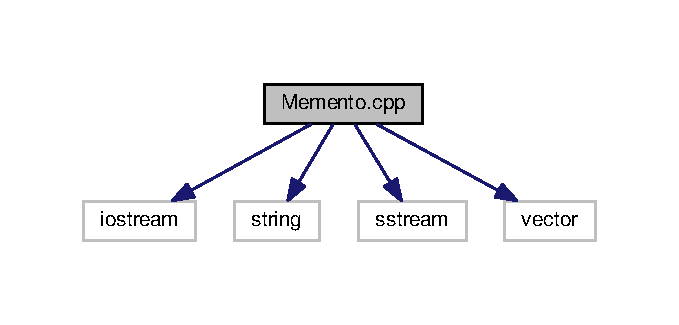
\includegraphics[width=326pt]{Memento_8cpp__incl}
\end{center}
\end{figure}
\subsection*{Classes}
\begin{DoxyCompactItemize}
\item 
class \hyperlink{classObject}{Object}
\item 
class \hyperlink{classMemento}{Memento}
\item 
class \hyperlink{classCommand}{Command}
\end{DoxyCompactItemize}
\subsection*{Functions}
\begin{DoxyCompactItemize}
\item 
{\footnotesize template$<$typename T $>$ }\\std\+::string \hyperlink{Memento_8cpp_a90503872144928016292aaa273e07678}{to\+String} (const T \&t)
\item 
int \hyperlink{Memento_8cpp_ae66f6b31b5ad750f1fe042a706a4e3d4}{main} ()
\end{DoxyCompactItemize}
\subsection*{Variables}
\begin{DoxyCompactItemize}
\item 
const std\+::string \hyperlink{Memento_8cpp_a549853b5d8df8cf60e8d275a4df73b54}{N\+A\+ME} = \char`\"{}Object\char`\"{}
\end{DoxyCompactItemize}


\subsection{Function Documentation}
\index{Memento.\+cpp@{Memento.\+cpp}!main@{main}}
\index{main@{main}!Memento.\+cpp@{Memento.\+cpp}}
\subsubsection[{\texorpdfstring{main()}{main()}}]{\setlength{\rightskip}{0pt plus 5cm}int main (
\begin{DoxyParamCaption}
{}
\end{DoxyParamCaption}
)}\hypertarget{Memento_8cpp_ae66f6b31b5ad750f1fe042a706a4e3d4}{}\label{Memento_8cpp_ae66f6b31b5ad750f1fe042a706a4e3d4}

\begin{DoxyCode}
99 \{
100     \textcolor{keywordtype}{int} i;
101     std::cout << \textcolor{stringliteral}{"Please enter an integer: "};
102     std::cin >> i;
103     \hyperlink{classObject}{Object} *\textcolor{keywordtype}{object} = \textcolor{keyword}{new} \hyperlink{classObject}{Object}(i);
104     
105     \hyperlink{classCommand}{Command} *commands[3];
106     commands[1] = \textcolor{keyword}{new} \hyperlink{classCommand}{Command}(\textcolor{keywordtype}{object}, &\hyperlink{classObject_a7e43ddd2f4647f67ba9d6f18dd24bf77}{Object::doubleValue});
107     commands[2] = \textcolor{keyword}{new} \hyperlink{classCommand}{Command}(\textcolor{keywordtype}{object}, &\hyperlink{classObject_a406add870a5642dc0d931aec975288f9}{Object::increaseByOne});
108     
109     std::cout << \textcolor{stringliteral}{"0.Exit,  1.Double,  2.Increase by one,  3.Undo,  4.Redo: "};
110     std::cin >> i;
111     
112     \textcolor{keywordflow}{while} (i != 0)
113     \{
114         \textcolor{keywordflow}{if} (i == 3)
115             \hyperlink{classCommand_a31a6d34a1d61f7cd994075a852714d3c}{Command::undo}();
116         \textcolor{keywordflow}{else} \textcolor{keywordflow}{if} (i == 4)
117             \hyperlink{classCommand_ac807fae3326e22c02edc737708f9b288}{Command::redo}();
118         \textcolor{keywordflow}{else} \textcolor{keywordflow}{if} (i > 0 && i <= 2)
119             commands[i]->\hyperlink{classCommand_a1f73a16e8706aec4c4db746f710b88d9}{execute}();
120         \textcolor{keywordflow}{else}
121         \{
122             std::cout << \textcolor{stringliteral}{"Enter a proper choice: "};
123             std::cin >> i;
124             \textcolor{keywordflow}{continue};
125         \}
126         std::cout << \textcolor{stringliteral}{"   "} << \textcolor{keywordtype}{object}->getValue() << \textcolor{stringliteral}{"  "} << \textcolor{keywordtype}{object}->getName() << \textcolor{stringliteral}{"  "} << \textcolor{keywordtype}{object}->getDecimal
      () << std::endl;
127         std::cout << \textcolor{stringliteral}{"0.Exit,  1.Double,  2.Increase by one,  3.Undo,  4.Redo: "};
128         std::cin >> i;
129     \}
130 \}\end{DoxyCode}


Here is the call graph for this function\+:
\nopagebreak
\begin{figure}[H]
\begin{center}
\leavevmode
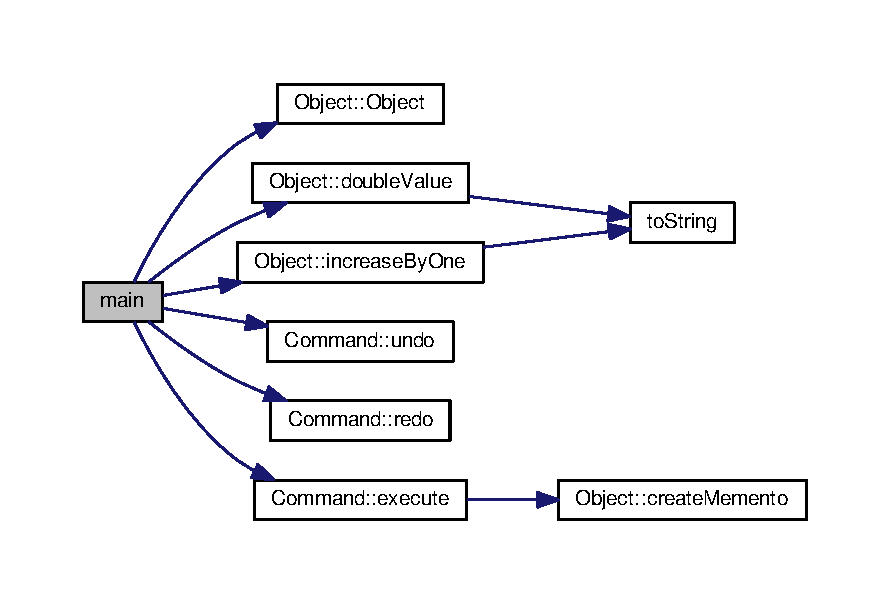
\includegraphics[width=350pt]{Memento_8cpp_ae66f6b31b5ad750f1fe042a706a4e3d4_cgraph}
\end{center}
\end{figure}


\index{Memento.\+cpp@{Memento.\+cpp}!to\+String@{to\+String}}
\index{to\+String@{to\+String}!Memento.\+cpp@{Memento.\+cpp}}
\subsubsection[{\texorpdfstring{to\+String(const T \&t)}{toString(const T &t)}}]{\setlength{\rightskip}{0pt plus 5cm}template$<$typename T $>$ std\+::string to\+String (
\begin{DoxyParamCaption}
\item[{const T \&}]{t}
\end{DoxyParamCaption}
)}\hypertarget{Memento_8cpp_a90503872144928016292aaa273e07678}{}\label{Memento_8cpp_a90503872144928016292aaa273e07678}

\begin{DoxyCode}
9                                 \{
10     std::stringstream ss;
11     ss << t;
12     \textcolor{keywordflow}{return} ss.str();
13 \}
\end{DoxyCode}


\subsection{Variable Documentation}
\index{Memento.\+cpp@{Memento.\+cpp}!N\+A\+ME@{N\+A\+ME}}
\index{N\+A\+ME@{N\+A\+ME}!Memento.\+cpp@{Memento.\+cpp}}
\subsubsection[{\texorpdfstring{N\+A\+ME}{NAME}}]{\setlength{\rightskip}{0pt plus 5cm}const std\+::string N\+A\+ME = \char`\"{}Object\char`\"{}}\hypertarget{Memento_8cpp_a549853b5d8df8cf60e8d275a4df73b54}{}\label{Memento_8cpp_a549853b5d8df8cf60e8d275a4df73b54}

%--- End generated contents ---

% Index
\backmatter
\newpage
\phantomsection
\clearemptydoublepage
\addcontentsline{toc}{chapter}{Index}
\printindex

\end{document}
